% !TeX spellcheck = en_US
\documentclass[11pt, fleqn]{article}
%\usepackage{siunitx}
\usepackage{texfiles/SpeedyGonzales}
\usepackage{texfiles/MediocreMike}
\title{Changes to the Project Plan}
\date{}
\begin{document}
	\maketitle
	\noindent
	\vspace*{-1.4cm}
	\noindent
	\textbf{Project Title:} Fairness In Classification \newline \noindent
	\textbf{Group Members:} Oskar og Anders \newline  \noindent
	\textbf{Vejleder på engelsk:} Aase Feragen \noindent
	\\\\
	
	\noindent The original development of certain milestones and key achievements during the project writing process is visualized in the Gant chart shown below. 
	\begin{figure}[H]
		\centering
		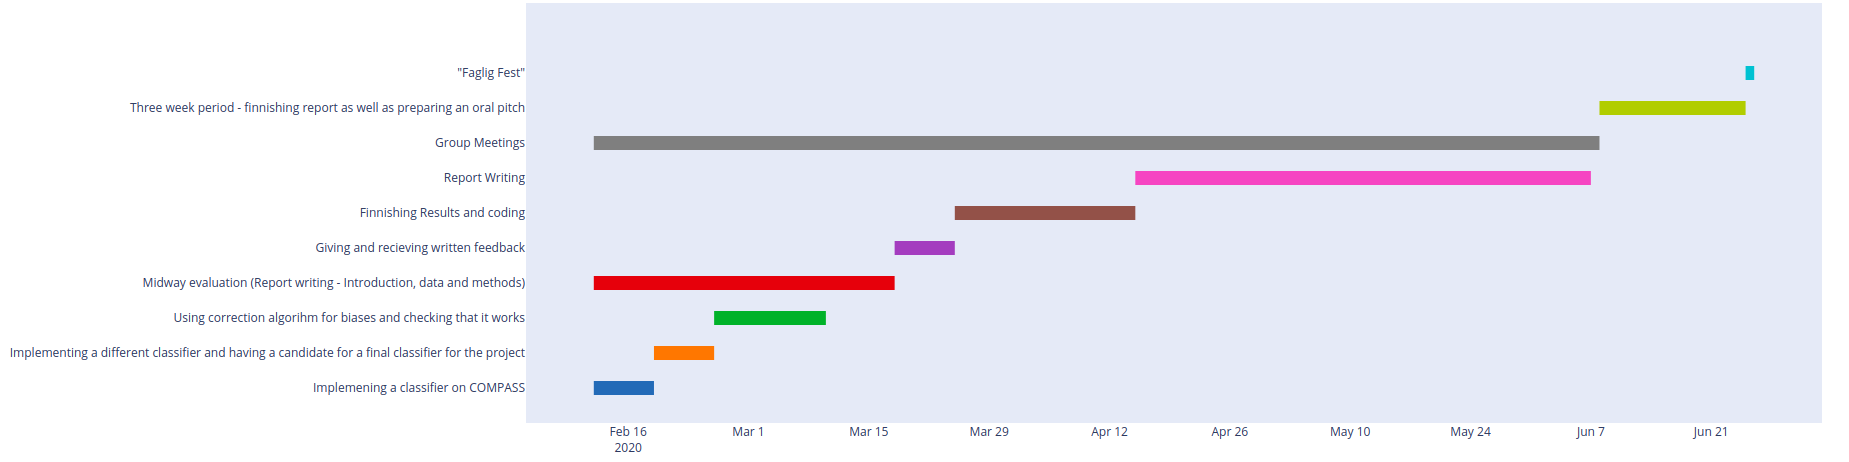
\includegraphics[width=\linewidth]{Gantt}
	\end{figure}

	Comparing this chart to the actual progress of the report writing, it is evident that it has been followed surprisingly well. As it seem wasteful to make strikingly similar classifers for the same task, the milestones of implementing the first classifier and creating the final classifer was merged into one. It also took longer, as some minor mistakes were made during the implementation. The bias correction algorithm took much longer to implement, as this turned out to be the same stage of the project as finishing results and coding. As such, this milestone was reached closer to the end of April than the middle of March. As we are in line with the further progression of the Gant chart (and since one of the last major milestones is writing the rest of the report), this will continue to be a guide moving forward.
	
	
	
\end{document}
